%!TEX TS-program = xelatex

% Шаблон документа LaTeX создан в 2018 году
% Алексеем Подчезерцевым
% В качестве исходных использованы шаблоны
% 	Данилом Фёдоровых (danil@fedorovykh.ru) 
%		https://www.writelatex.com/coursera/latex/5.2.2
%	LaTeX-шаблон для русской кандидатской диссертации и её автореферата.
%		https://github.com/AndreyAkinshin/Russian-Phd-LaTeX-Dissertation-Template

\documentclass[a4paper,14pt]{article}


%%% Работа с русским языком
\usepackage[english,russian]{babel}   %% загружает пакет многоязыковой вёрстки
\usepackage{fontspec}      %% подготавливает загрузку шрифтов Open Type, True Type и др.
\defaultfontfeatures{Ligatures={TeX},Renderer=Basic}  %% свойства шрифтов по умолчанию
\setmainfont[Ligatures={TeX,Historic}]{Times New Roman} %% задаёт основной шрифт документа
\setsansfont{Comic Sans MS}                    %% задаёт шрифт без засечек
\setmonofont{Courier New}
\usepackage{indentfirst}
\frenchspacing

\renewcommand{\epsilon}{\ensuremath{\varepsilon}}
\renewcommand{\phi}{\ensuremath{\varphi}}
\renewcommand{\kappa}{\ensuremath{\varkappa}}
\renewcommand{\le}{\ensuremath{\leqslant}}
\renewcommand{\leq}{\ensuremath{\leqslant}}
\renewcommand{\ge}{\ensuremath{\geqslant}}
\renewcommand{\geq}{\ensuremath{\geqslant}}
\renewcommand{\emptyset}{\varnothing}

%%% Дополнительная работа с математикой
\usepackage{amsmath,amsfonts,amssymb,amsthm,mathtools} % AMS
\usepackage{icomma} % "Умная" запятая: $0,2$ --- число, $0, 2$ --- перечисление

%% Номера формул
%\mathtoolsset{showonlyrefs=true} % Показывать номера только у тех формул, на которые есть \eqref{} в тексте.
%\usepackage{leqno} % Нумерация формул слева	

%% Перенос знаков в формулах (по Львовскому)
\newcommand*{\hm}[1]{#1\nobreak\discretionary{}
	{\hbox{$\mathsurround=0pt #1$}}{}}

%%% Работа с картинками
\usepackage{graphicx}  % Для вставки рисунков
\graphicspath{{images/}}  % папки с картинками
\setlength\fboxsep{3pt} % Отступ рамки \fbox{} от рисунка
\setlength\fboxrule{1pt} % Толщина линий рамки \fbox{}
\usepackage{wrapfig} % Обтекание рисунков текстом

%%% Работа с таблицами
\usepackage{array,tabularx,tabulary,booktabs} % Дополнительная работа с таблицами
\usepackage{longtable}  % Длинные таблицы
\usepackage{multirow} % Слияние строк в таблице
\usepackage{float}% http://ctan.org/pkg/float

%%% Программирование
\usepackage{etoolbox} % логические операторы


%%% Страница
\usepackage{extsizes} % Возможность сделать 14-й шрифт
\usepackage{geometry} % Простой способ задавать поля
\geometry{top=20mm}
\geometry{bottom=20mm}
\geometry{left=20mm}
\geometry{right=10mm}
%
%\usepackage{fancyhdr} % Колонтитулы
% 	\pagestyle{fancy}
%\renewcommand{\headrulewidth}{0pt}  % Толщина линейки, отчеркивающей верхний колонтитул
% 	\lfoot{Нижний левый}
% 	\rfoot{Нижний правый}
% 	\rhead{Верхний правый}
% 	\chead{Верхний в центре}
% 	\lhead{Верхний левый}
%	\cfoot{Нижний в центре} % По умолчанию здесь номер страницы

\usepackage{setspace} % Интерлиньяж
\onehalfspacing % Интерлиньяж 1.5
%\doublespacing % Интерлиньяж 2
%\singlespacing % Интерлиньяж 1

\usepackage{lastpage} % Узнать, сколько всего страниц в документе.

\usepackage{soul} % Модификаторы начертания

\usepackage{hyperref}
\usepackage[usenames,dvipsnames,svgnames,table,rgb]{xcolor}
\hypersetup{				% Гиперссылки
	unicode=true,           % русские буквы в раздела PDF
	pdftitle={Заголовок},   % Заголовок
	pdfauthor={Автор},      % Автор
	pdfsubject={Тема},      % Тема
	pdfcreator={Создатель}, % Создатель
	pdfproducer={Производитель}, % Производитель
	pdfkeywords={keyword1} {key2} {key3}, % Ключевые слова
	colorlinks=true,       	% false: ссылки в рамках; true: цветные ссылки
	linkcolor=black,          % внутренние ссылки
	citecolor=black,        % на библиографию
	filecolor=magenta,      % на файлы
	urlcolor=black           % на URL
}
\makeatletter 
\def\@biblabel#1{#1. } 
\makeatother
\usepackage{cite} % Работа с библиографией
%\usepackage[superscript]{cite} % Ссылки в верхних индексах
%\usepackage[nocompress]{cite} % 
\usepackage{csquotes} % Еще инструменты для ссылок

\usepackage{multicol} % Несколько колонок

\usepackage{tikz} % Работа с графикой
\usepackage{pgfplots}
\usepackage{pgfplotstable}

% ГОСТ заголовки
\usepackage[font=small]{caption}
%\captionsetup[table]{justification=centering, labelsep = newline} % Таблицы по правобу краю
%\captionsetup[figure]{justification=centering} % Картинки по центру


\newcommand{\tablecaption}[1]{\addtocounter{table}{1}\small \begin{flushright}\tablename \ \thetable\end{flushright}%	
\begin{center}#1\end{center}}

\newcommand{\imref}[1]{рис.~\ref{#1}}

\usepackage{multirow}
\usepackage{spreadtab}
\newcolumntype{K}[1]{@{}>{\centering\arraybackslash}p{#1cm}@{}}


\usepackage{xparse}
\usepackage{fancyvrb}

\RecustomVerbatimCommand{\VerbatimInput}{VerbatimInput}
{
	fontsize=\footnotesize    
}

\usepackage{tocloft}
\renewcommand{\cftsecleader}{\cftdotfill{\cftdotsep}}
\begin{document} % конец преамбулы, начало документа
	\begin{titlepage}
	\begin{center}
 		ФЕДЕРАЛЬНОЕ  ГОСУДАРСТВЕННОЕ АВТОНОМНОЕ \\
		ОБРАЗОВАТЕЛЬНОЕ УЧРЕЖДЕНИЕ ВЫСШЕГО ОБРАЗОВАНИЯ\\
		«НАЦИОНАЛЬНЫЙ ИССЛЕДОВАТЕЛЬСКИЙ УНИВЕРСИТЕТ\\
		«ВЫСШАЯ ШКОЛА ЭКОНОМИКИ»
	\end{center}
	
	\begin{center}
		\textbf{Московский институт электроники и математики}
		
		\textbf{им. А.Н.Тихонова НИУ ВШЭ}
		
		\vspace{2ex}
		
		\textbf{Департамент компьютерной инженерии}
	\end{center}
	\vspace{1ex}	
	
	\begin{center}
		Курс «Системное проектирование цифровых устройств»
	\end{center}	
	
	
	\begin{center}
	\textbf{ОТЧЕТ\\
		ПО ЛАБОРАТОРНОЙ РАБОТЕ №5
	}
	\end{center}	

	\begin{center}
		Тема работы: «Обработка звука на ПЛИС»
	\end{center}

	\vspace{2ex}

	\begin{flushright}
		\textbf{Выполнили:}
		
		\vspace{2ex}
		
		Студенты группы БИВ174
		
		Бригада №5
		
		\vspace{2ex}
		
		Подчезерцев Алексей Евгеньевич
		
		Солодянкин Андрей Александрович
		\vspace{2ex}
		
		\textbf{Принял:}
		
		асс. МИЭМ НИУ ВШЭ
		
		Американов А.А.
		
	\end{flushright}

	\vfill
	\begin{center}
		Москва \the\year \, г.
	\end{center}
	
\end{titlepage}
\addtocounter{page}{1}
	\tableofcontents
	\pagebreak
	\section{Задание}
	
	\begin{enumerate}
		
		\item Изучить раздел 5.2 Audio Recording and Playing в \_DE1-SoC\_User\_manual.pdf.
		
		\item Модифицировать файл DE1\_SoC\_Audio.bat под выполнение на вашем компьютере.
		
		\item Запустить проект и продемонстрировать его работу.
		
		\item Запустить и загрузить в SOPC аппаратную часть проекта. Отобразить в отчете, структуру NIOS ядра, описать какие компоненты к ядру подключены и для чего.
		
		\item Запустить Nios II Software Build Tools for Eclipse. Отобразить в отчете схему организации программной части проекта. Найти точку входа в проект. Уметь объяснить назначение используемых функций.
		
		\item Изучить раздел 5.3 Karaoke Machine в \_DE1-SoC\_User\_manual.pdf.
		
		\item Модифицировать файл DE1\_SoC\_i2sound.bat под выполнение на вашем компьютере.
		
		\item Запустить проект и продемонстрировать его работу.
		
		\item Описать отличия проекта SPDS\_Lab\_8\_DE1\_SoC\_i2sound от \\ SPDS\_Lab\_8\_DE1\_SoC\_Audio в их реализации.
		
		\item Модифицировать пример из раздела 5.2 так, чтобы с помощью кнопок SW6 – SW9 можно было регулировать громкость воспроизведения. А кнопкой 1 включать пищалку.
		
	\end{enumerate}

	%{\small \VerbatimInput{../03_syn_pow_5_single_cycle_always/pow_5_single_cycle_always.v}}
	
	\section{Выполнение работы}
	
	На рис. \ref{fig:shemeqsys} приведена блок схема, показывающая связь между компонентами, подключенными к ядру.
	На рис. \ref{fig:qsys} скриншот связи между компонентами из программы Platform Designer.
	
	\begin{enumerate}
		
		\item Nios II -- процессорное ядро;
		
		\item JTAG UART -- компонент, позволяющий взаимодействовать плате и ПК;
		
		\item PLL -- компонент управляющий записью в память памятью;
		
		\item SDRAM Controller -- компонент управляющий памятью;
		
		\item SDRAM0 -- память, на которой храниться записанный голос;
		
		\item On Chip Memory -- память с программой;
		 
		\item AUDIO Controller -- компонент для взаимодействия с кодеком;
		
		\item AUDIO -- кодек преобразующий сигнал с линейного входа в цифровой сигнал и наоборот;
		
		\item PIO Controller -- компонент, позволяющий общаться с периферией платы;
		
		\item System Interconnect Fabric -- шина данных.
		
	\end{enumerate}
	
	\begin{figure}[H]
		\centering
		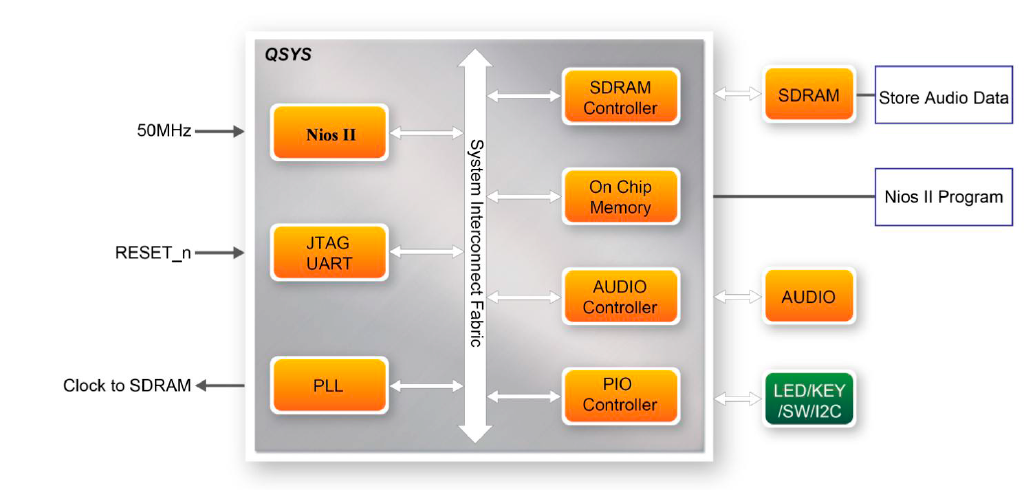
\includegraphics[width=0.7\linewidth]{images/sheme_qsys}
		\caption{Блок диаграмма связи между компонентами}
		\label{fig:shemeqsys}
	\end{figure}

	\begin{figure}[H]
		\centering
		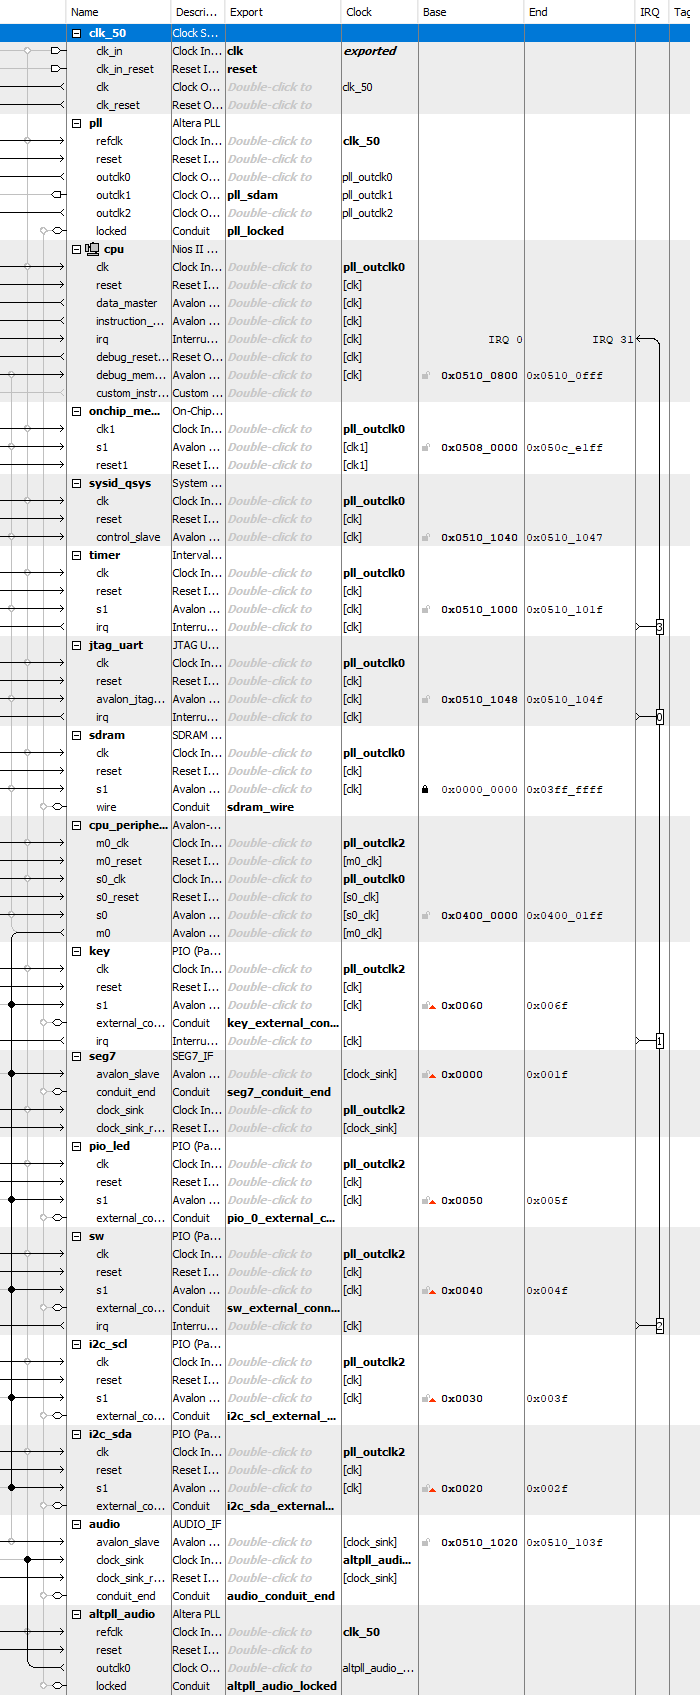
\includegraphics[width=0.55\linewidth]{images/QSYS1}
		\caption{Все компоненты периферии}
		\label{fig:qsys}
	\end{figure}

	Программная часть состоит из нескольких файлов, запускается файл $main.c$, в нем точкой входа является функция main.
	головные файлы остальных подгружаемых библиотек: $my\_includes.h$, $AUDIO.h$, $LED.h$, $SEG7.h$ и $<math.h>$.
	
	На рис. \ref{fig:shemeqsys2} представлена блок схема для Karaoke machine.
	
	\begin{figure}[H]
		\centering
		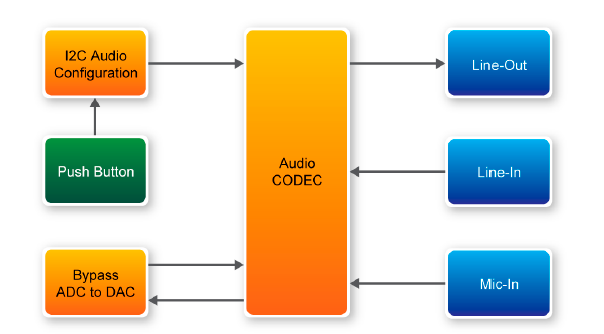
\includegraphics[width=0.7\linewidth]{images/sheme_qsys_2}
		\caption{Блок диаграмма для Karaoke machine}
		\label{fig:shemeqsys2}
	\end{figure}
	
	Проект i2sound реализован на самом железе платы, включая кодек.
	Данные с линейных входов поступают сразу к нему, складываются и в преобразованном виде отправляются на линейный выход.
	При этом к кодеку подключены различные элементы управления.

	Проект Audio реализован на готовом ядре процессора.
	Кодек реализован в программном виде и в виде компонента присоединен через шину к процессору.
	
	При этом в проектах используются одинаковый интерфейс i2c.	
	

	\section{Самостоятельная работа}
	
	Модифицировать пример из раздела 5.2 так, чтобы с помощью кнопок SW6 – SW9 можно было регулировать громкость воспроизведения. 
	А кнопкой 1 включать пищалку.
	
	Пример был модифицирован.

	\section{Выводы по работе}
	
	В ходе работы было получено представление о звуке в цифровых устройствах.
	Был получен опыт в написании и анализе кода на языке С.
	Был получен опыт генерации звука при помощи ПЛИС и языка С.
	Было изучено хранение звука в памяти ПЛИС.
	Был получен опыт в обработке звука пр помощи компонентов в $Platform Designer$.
	Был изучен способ программного повышения громкости в языке С.
	Итоговый проект был собран и загружен на плату.

	
	\newpage 
	\renewcommand{\refname}{{\normalsize Список использованных источников}} 
	\centering 
	\begin{thebibliography}{9} 
		\addcontentsline{toc}{section}{\refname} 
		\bibitem{Harris} Хэррис Д. М., Хэррис С. Л. Цифровая схемотехника и архитектура компьютера. – 2015.
	\end{thebibliography}
	
\end{document} % конец документа
